\documentclass[]{article}
\usepackage{fullpage}
\usepackage[authoryear]{natbib}
\usepackage{setspace}
    \doublespacing
\usepackage{hyperref}
\hypersetup{
    colorlinks,
    citecolor=black,
    filecolor=black,
    linkcolor=cyan,
    urlcolor=cyan
}
\usepackage{amssymb,amsmath}
\usepackage{bm}
\usepackage{dcolumn}
\usepackage{booktabs}
\usepackage{url}
\usepackage{tikz}
\usepackage{todonotes}
\usepackage[utf8]{inputenc}
\usepackage{graphicx}
\usepackage{longtable}
\usepackage{todonotes}
\usepackage{lscape}
\usepackage{float}

\usepackage[margins]{trackchanges}


\title{Can You Stop the Fire Before it Burns Down the Block? Central banks and the fiscal costs of financial crises}

\author{Christopher Gandrud \\ \emph{City University London} \\ \emph{Hertie School of Governance}\footnote{Christopher Gandrud is Lecturer in Quantitative International Political Economy at City University London and Post-doctoral fellow at the Hertie School of Governance. Please contact him at Rhind Building, City University London, EC1V 0HB, London, United Kingdom
(\href{mailto:christopher.gandrud@city.ac.uk}{\nolinkurl{christopher.gandrud@city.ac.uk}}). Mark Hallerberg is Professor of Public Management and Political Economy at the Hertie School of Governance, Friedrichstrasse 180, Berlin 10117, Germany (\href{mailto:hallerberg@hertie-school.org}{\nolinkurl{hallerberg@hertie-school.org}}). This work was supported by the Deutsche Forschungsgemeinschaft under grant number HA5996/2-1. Replication material can be found at: \url{https://github.com/christophergandrud/ela_fiscal_costs}.}
\and
Mark Hallerberg \\ \emph{Hertie School of Governance}}

\begin{document}

\maketitle

\addeditor{MH}
\addeditor{CG}

\noindent \textbf{Working draft prepared for the 2016 International Political Economy Society Conference. Comments welcome.}

\begin{abstract}
Effective emergency liquidity assistance (ELA) can play an important role in reducing the severity of a financial crisis. It can come from an international actor, such as the European Union or the IMF, or a domestic actor, often a country's central bank.
 We seek to explain when a government approaches an international funder by exploring the conditioning effects of central banks. Without ELA, banks in a credit crunch might be forced to sell-off their assets in fire sales, depressing asset prices, and possibly leading to bank failures. We propose a framework to understand
 the amount, conditions, and timing of ELA. We consider the role
of mandates, e.g. for price stability versus financial
stability for setting an ``upper bound'' on what ELA central banks could provide. We also argue that the international environment--currency regime commitments, the possibility of assistance from international institutions and other countries, and currency crisis contagion--affects the ability of central banks to provide ELA. Finally, we contend that the fiscal accounting regime affects the decision to use ELA. If the government finance accounting regime treats ELA as off-budget, then politicians push to use this option. Central banks that are more concerned with price stability and their reputation, could push back. We find evidence for this process with both a cross-country analysis of ELA and case studies using newly released documents from the United Kingdom, Ireland, and the European Central Bank. We relate these decisions to requests for liquidity assistance from international financial institutions in the first place.
\end{abstract}

\textbf{Word count:} -----

\section{Introduction}

\section{Our argument: politicians and central banks}

\todo[inline]{This is just from the book proposal}

The accounting of central bank actions also affects politicians' choices. Often central bank emergency liquidity assistance (ELA) is treated as off of the fiscal balance sheet, thus decreasing the need for politicians to respond in ways that would increase the debt. For example, in the United Kingdom in 2009, the Bank of England intentionally did not report the scale of its emergency liquidity assistance, and it has a rule to make such assistance known only at a time when its reporting would not hurt the bank that received the assistance.\footnote{See UK Parliament 2009, ``Reporting Contingent Liabilities to Parliament.'' Accessed at \url{http://www.publications.parliament.uk/pa/cm200910/cmselect/cmtreasy/181/18103.htm} August 2015.} The extent to which the accounting regime recognizes such operations affects politicians' incentives to push the central bank to extend such assistance.

Central bank ELA operations are at the very least implicitly guaranteed by their governments, if not explicitly guaranteed. If
a central bank extends ELA, but banks still default and their collateral is not sufficient to cover their default, then a central bank could become insolvent. It would need the government to recapitalized it in order for the monetary and payment system, and therefore the economy, to continue operating. Alternatively, a central bank could create money to cover its obligations, but this would hinder its monetary policy objectives as it could create inflation. Accounting rules can shape how fiscal backstops affect the debt and therefore how attractive they are to politicians. For example, the Bank of England informed the Treasury in October 2008 that, without a public guarantee, the Bank would effectively provide less emergency assistance and impose higher costs on banks. Politicians were reluctant to extend such a guarantee if it would be made public immediately.\footnote{From the Bank of England’s Transactions Sub­committee of Court Minutes available
 at: \url{http://www.bankofengland.co.uk/archive/Documents/archivedocs/codm/20072009/transactionscom.pdf}. Accessed August 2015}
 Ultimately, the guarantees were made and they were publicly disclosed a year after the fact, thus skirting the edges of an accounting regime that would have made potential costs more transparent.

Another part of the rules concerns the differences between cash and accrual accounting. Under cash accounting, costs are only recorded when they are paid. Under accrual accounting, expected costs are entered on the books immediately. Under cash accounting, policies such as Ireland’s 2010 “promissory notes”6 are an effective way to shift costs into the future and are therefore attractive to elected officials. Under accrual accounting rules they are not.

\begin{figure}
    \caption{Monetary Policy Manoeuvrability and the Costs of Resolving Financial Crises}
    \label{mpcost}
    \centering
    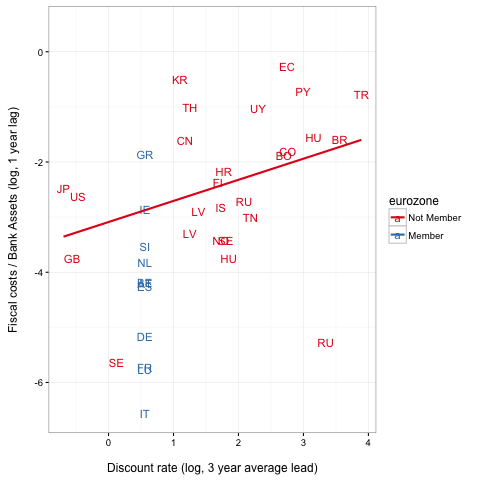
\includegraphics[scale=0.5]{figures/DiscountRate_CostsStnd.png}

\end{figure}

\section{Case studies}

\subsection{Bank of England--NedCo}


\subsection{Central Bank of Ireland--Letter of Comfort}


\subsection{European Central Bank}


\section{Large-n}


\section{Conclusions}


\end{document}
